
\section{Introduction}
In the enchanting world of wizardry, the art of spellcasting stands as a cornerstone of magical prowess. This chapter delves into the intricate and captivating practice of weaving spells, exploring the fundamental principles that govern the casting of magical incantations. From the flick of a \gls{wand} to the resonance of ancient words \cite{ancientspellcraft2018}, we embark on a journey through the essence of spellcasting.

In the enchanting world of wizardry, casting a \gls{spell} is a fundamental practice. Wizards often brew mystical potions known as \glspl{elixir} to enhance their magical abilities. The chapter also explores the mystical art of \gls{ap}, allowing wizards to traverse otherworldly realms.

\section{Foundations of Spellcraft}

The foundation of spellcraft lies in the understanding of magical elements, gestures, and words. Wizards have long sought to unravel the secrets of effective spellcasting, and this section examines the core components that contribute to the success of a spell. From the precise movement of a \gls{wand} \cite{wandmovements2019} to the linguistic nuances of incantations \cite{spellweaver2022}, each element plays a vital role in shaping the magical forces at work.

The \gls{crystal} is a powerful artifact for casting spells, and the \gls{enchant} is a mysterious ritual for channeling arcane energies. 
The \gls{scroll} holds ancient wisdom and linguistic secrets \cite{magiclanguage2021}.

Magical spells are the cornerstone of wizardry. The process involves intricate wand movements, precise incantations, and a deep connection with the magical energies that permeate the universe. For instance, a skilled wizard might cast a protective shield by waving their wand in a specific pattern and uttering the incantation "Protego Maxima!" The effectiveness of the spell is influenced by the wizard's mastery of the magical language and the energy channeled into the wand.

\section{Classifying Magical Spells}

\begin{figure}
    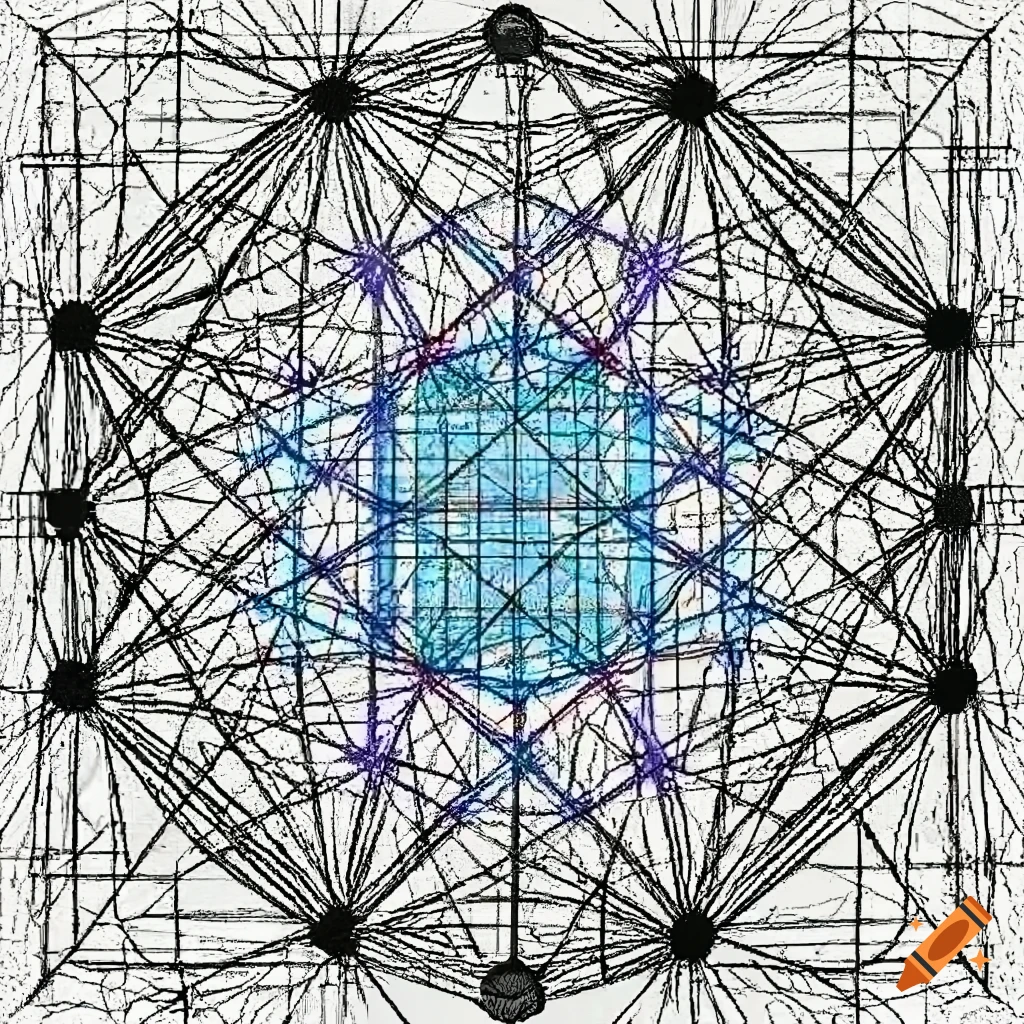
\includegraphics[width=\textwidth]{fig/img1.png}
    \caption{The Spellweaver Matrix is a visual representation of the intricate relationships between \gls{wand} movements, linguistic nuances \cite{linguisticnuances2016}, and \gls{spell}efficacy. This matrix, created by Grand Sorcerer Thaddeus Spellweaver, illustrates the harmonious dance of these elements, offering a guide for aspiring spellcasters to enhance the potency of their incantations.}
    \label{fig:img1}
  \end{figure}

Magical \glspl{spell}come in a myriad of forms, each with its own purpose and properties. This section categorizes \glspl{spell}based on their intent, from protective charms to offensive hexes. Through a comprehensive classification system (Fig.~\ref{fig:img1}), we aim to unravel the underlying principles that define the nature of different spells. The taxonomy presented here serves as a guide to aspiring wizards seeking to navigate the vast repertoire of magical knowledge.

In the pursuit of mastering spellcasting, wizards often measure their progress in magical currency. A powerful spell might require the expenditure of magical resources, denominated in galleons (\si{\galleon}), sickles (\si{\sickle}), and knuts (\si{\knut}). For example, a complex transformation spell may consume \SI{10}{\galleon}s, \SI{5}{\sickle}s, and \SI{20}{\knut}s worth of magical energy.

\section{Experimental Spellcasting}
To gain deeper insights into the art of spellcasting, wizards often engage in experimental practices. This section explores the methods employed in experimental spellcasting, including controlled environments, \gls{spell}modification, and the study of magical feedback. By pushing the boundaries of traditional spellcraft, wizards can discover new applications, uncover hidden properties, and contribute to the ever-evolving tapestry of magical arts.

Wizards also experiment with unconventional spellcasting techniques, such as incorporating unicorn hairs (\SI{0.5}{\unicornhair} per spell) into their wands. The presence of unicorn hair enhances the purity and potency of the magical incantation. As wizards delve into the complexities of spellcasting, they explore the synergies between various magical components and the impact on the outcome of their spells.

\section{The Alchemy of Incantations}
The spoken word holds immense power in the realm of spellcasting. This section delves into the alchemy of incantations, examining the phonetic structures and mystical resonance of words. Wizards often spend years perfecting their pronunciation and mastering the linguistic subtleties that enhance the potency of their spells. The chapter explores the intersection of language and magic, shedding light on the transformative nature of incantations.

The art of spellcasting is a lifelong journey for wizards, with each incantation representing a step towards unlocking the mysteries of the magical world.

\section{Conclusion}
As we conclude our exploration into the art of spellcasting, we reflect on the rich tapestry of magical knowledge uncovered in this chapter. From the foundational elements to the experimental realms, spellcasting remains a captivating and dynamic aspect of wizardry. The insights gained here serve as a stepping stone for further magical research, encouraging wizards to continue pushing the boundaries of their craft and unlocking the boundless potential that lies within the art of spellcasting.

